\newcommand{\e}{\`e }
\newcommand{\E}{\`E }
\newcommand{\nec}{n\'e }
\newcommand{\Nec}{N\'e }
\newcommand{\cioe}{cio\`e }
\newcommand{\Cioe}{Cio\`e }
\newcommand{\piu}{pi\`u }
\newcommand{\Piu}{Pi\`u }
\newcommand{\cosi}{cos\`{\i} }
\newcommand{\Cosi}{Cos\`{\i} }
\newcommand{\poiche}{poich\'e }
\newcommand{\Poiche}{Poich\'e }
\newcommand{\purche}{purch\'e }
\newcommand{\Purche}{Purch\'e }
\newcommand{\perche}{perch\'e }
\newcommand{\Perche}{Perch\'e }

\newcommand{\st}[1]{{\tau[\![{#1}]\!]}}
\newcommand{\se}[2]{{\tau^{#1}[\![{#2}]\!]}}
\newcommand{\inter}[1]{{[\![{#1}]\!]}}
\newcommand{\gen}[1]{{\gamma[\![{#1}]\!]}}
\newcommand{\gentwo}[2]{{\gamma^{{#1}}[\![{#2}]\!]}}
\newcommand{\gentwotwo}[2]{{\gamma^{{#1}}\left[\!\left[{#2}\right]\!\right]}}
\newcommand{\gentest}[1]{{\gamma^{\mathit{test}}[\![{#1}]\!]}}
\newcommand{\sig}[2]{{\tau^{#1}[\![{#2}]\!]}}
\newcommand{\nullable}{\mathsf{nullable}}
\newcommand{\first}{\mathsf{first}}
\newcommand{\follow}{\mathsf{follow}}
\newcommand{\lfp}{\mathit{lfp}}
\newcommand{\idot}{.\,}
\newcommand{\vars}[1]{{\mathsf{vars}[\![{#1}]\!]}}
\newcommand{\declared}[1]{{\mathsf{declared}[\![{#1}]\!]}}
\newcommand{\used}[1]{{\mathsf{used}[\![{#1}]\!]}}
\newcommand{\cdc}{\vdash^{\mathsf{cdc}}}

\definecolor{lightgrey}{rgb}{0.8,0.8,0.8}

\newcommand{\javatip}[1]{
  \begin{center}
  \begin{tabular}{cc}
  \hspace*{-0.5cm}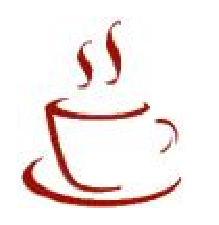
\epsfig{file = javacup.ps, width = 1.3cm}\hspace*{0.5cm} &
  {\small\colorbox{lightgrey}{\begin{minipage}{13cm}{#1}\end{minipage}}}
  \end{tabular}
  \end{center}
}

\newcommand{\greycomment}[1]{
  \begin{center}
  \begin{tabular}{cc}
  \hspace*{-0.5cm}
\epsfig{file = questionmark.ps, width = 1.3cm}\hspace*{0.5cm}
  {\small\colorbox{lightgrey}{\begin{minipage}{13cm}{#1}\end{minipage}}}
  \end{tabular}
  \end{center}
}

\newcommand{\greycommens}[1]{
  \begin{center}
  \hspace*{-0.5cm}
\epsfig{file = questionmark.ps, width = 1.3cm}\hspace*{0.5cm}
  {\small\colorbox{lightgrey}{\begin{minipage}{13cm}{#1}\end{minipage}}}
  \end{center}
}

\theoremstyle{definition}
\newtheorem{definition}{Definizione}
\newtheorem{proposition}{Proposizione}
\newtheorem{exercise}{Esercizio}